\documentclass{article}
\usepackage[utf8]{inputenc}
\usepackage[margin=0.75in]{geometry}
\usepackage{enumerate}
\usepackage{amsmath}
\usepackage{amsfonts} 
\usepackage{amssymb}
\usepackage{amsthm}
\usepackage{mathtools}
\usepackage{float}
\usepackage{array}
\usepackage{makecell}
\usepackage{commath}
\usepackage{verbatim}

\DeclarePairedDelimiter{\ceil}{\lceil}{\rceil}

\renewcommand\theadalign{bc}
\renewcommand\theadfont{\bfseries}
\renewcommand\theadgape{\Gape[4pt]}
\renewcommand\cellgape{\Gape[4pt]}

\newcommand{\N}{\mathbb{N}}
\newcommand{\Z}{\mathbb{Z}}
\newcommand{\Q}{\mathbb{Q}}
\newcommand{\C}{\mathbb{C}}
\newcommand{\R}{\mathbb{R}}
\newcommand{\F}{\mathbb{F}}
\newtheorem{theorem}{Theorem}
\newtheorem{corollary}{Corollary}[theorem]
\newtheorem{definition}{Definition}[theorem]
\newtheorem{lemma}[theorem]{Lemma}
\newtheorem*{remark}{Remark}
\newcommand{\cdotscalar}{\;\widetilde{\cdot}\;}
\newcommand{\vectorplus}{\;\widetilde{+}\;}
\newcommand{\Span}{\text{Span}}
\newcommand{\Null}{\text{Null}}
\newcommand{\Range}{\text{Range}}
\newcommand{\D}{\frac{d}{\dif x}}

\renewcommand{\epsilon}{\varepsilon}
\renewcommand{\phi}{\varphi}

\newcommand{\Or}{\mbox{ OR }}
\renewcommand{\And}{\mbox{ AND }}
\newcommand{\Not}{\mbox{NOT }}
\newcommand{\Iff}{\mbox{ IFF }}

\newcommand{\Width}{\textup{width}}
\newcommand{\Mesh}{\textup{mesh}}
\newcommand{\Int}{\textup{Int}}
\newcommand{\Ext}{\textup{Ext}}
\newcommand{\Bd}{\textup{Bd}}
\newcommand{\argmax}{\textup{argmax}}


\newcommand\widebar[1]{\mathop{\overline{#1}}}
\newcommand*\closure[1]{\widebar{#1}}

\newcommand\Ball[2]{U(#1; #2)}

\begin{document}

\section*{Question 1: Backpropagation}

\begin{enumerate}[(a)]
    \item Here's the computation graph for the given network:
    
    \begin{figure}[H]
        \centering
        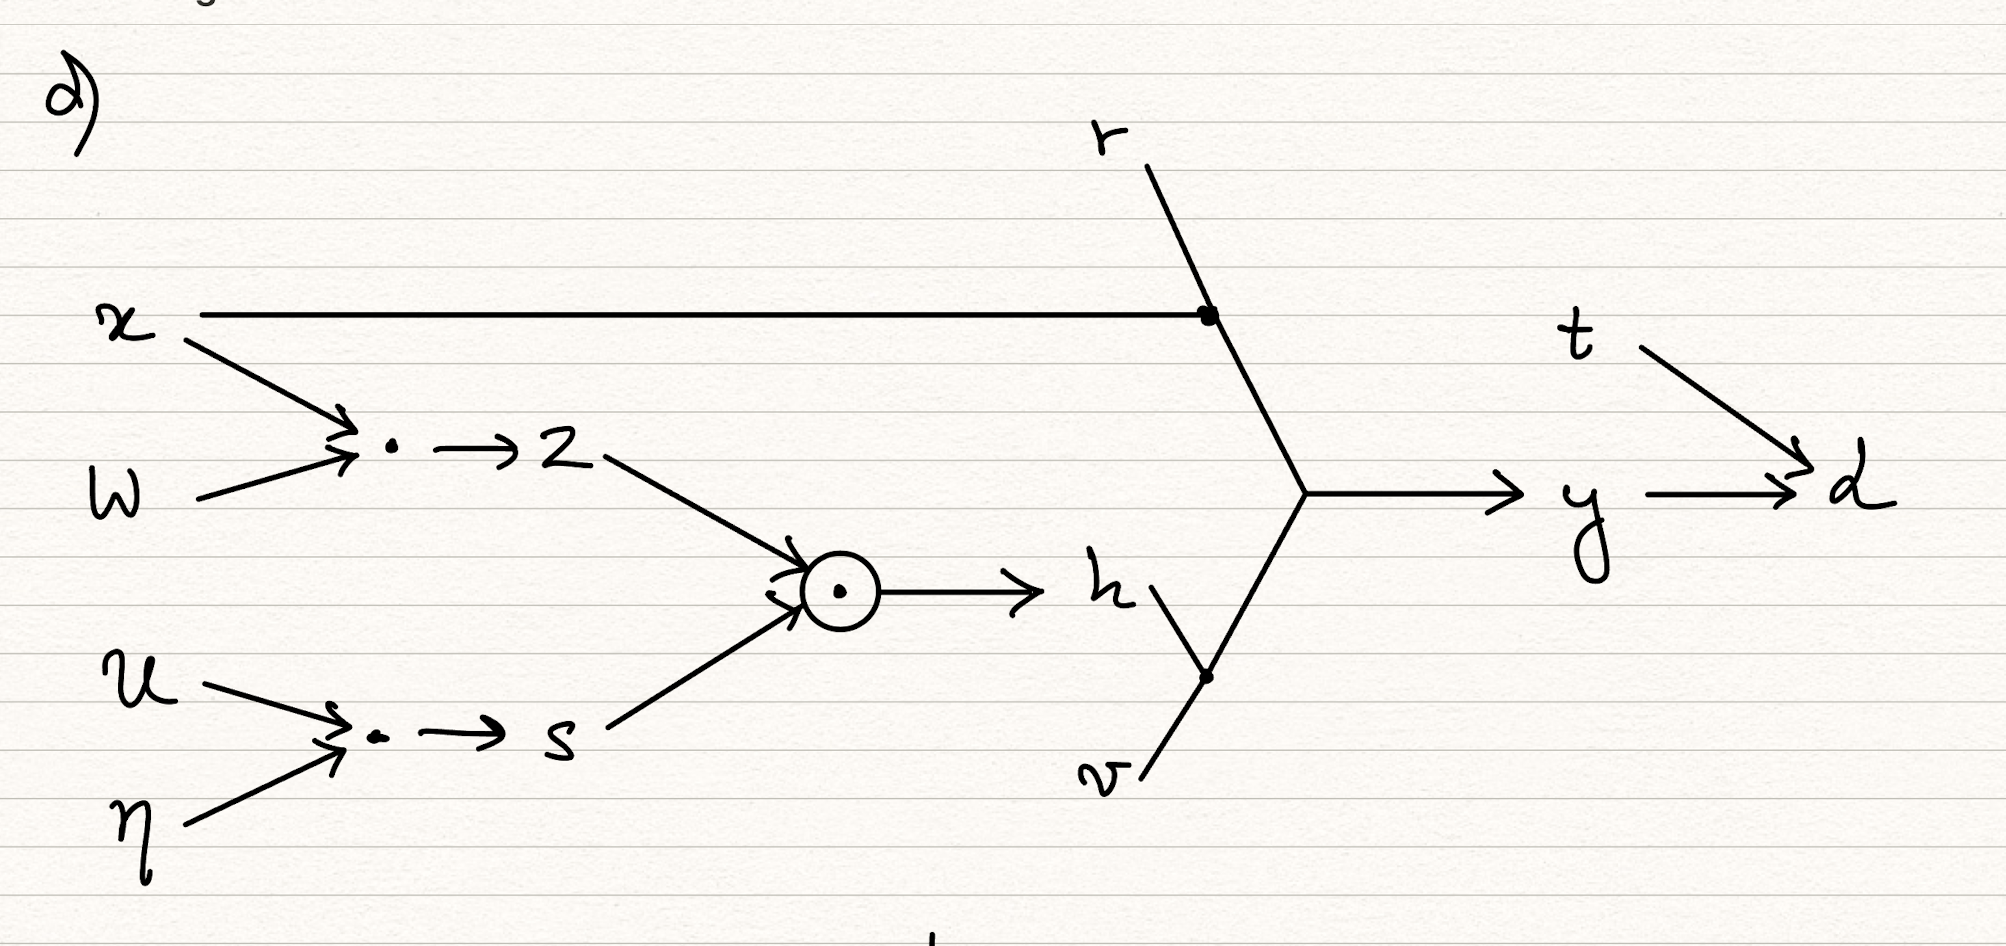
\includegraphics[width=0.8\textwidth]{../q1_graph.png}
    \end{figure}

    \item We proceed as follows, first computing both quantities and showing equality: 
    
    \begin{align*}
        \frac{\dif}{\dif x} \sigma(x) &= \frac{\dif}{\dif x} \frac{1}{1 + e^{-x}} \\
        &= -1 \cdot (1 + e^{-x})^{-2} \cdot -1 \cdot e^{-x}\\
        &= \frac{e^{-x}}{(1 + e^{-x})^2} \\
    \end{align*}

    \begin{align*}
        \sigma(x) (1 - \sigma(x)) &= \frac{1}{1 + e^{-x}} \left(1 - \frac{1}{1 + e^{-x}}\right) \\
        &= \frac{1}{1 + e^{-x}} \left(\frac{e^{-x}}{1 + e^{-x}}\right) \\
        &= \frac{e^{-x}}{(1 + e^{-x})^2} \\
    \end{align*}

    showing that

    \[\sigma'(x) = \sigma(x) (1 - \sigma(x))\]

    \item First, let's define the intermediate quantity \[u = v^T h + r^T x\]
    such that \[y = \sigma(u)\]
    
    Then, let's list all partial derivatives needed in the calculation:
    
    \begin{align*}
        \frac{\partial \mathcal{L}}{\partial y} &= \frac{t}{y} - \frac{1 - t}{1 - y}\\
        \frac{\partial \mathcal{L}}{\partial t} &= \log(y) - \log(1 - y)\\[1em]
        \frac{\partial y}{\partial u} &= \sigma(u) (1 - \sigma(u))\\[1em]
        \frac{\partial u}{\partial v} &= h^T\\
        \frac{\partial u}{\partial h} &= v^T\\
        \frac{\partial u}{\partial r} &= x^T\\
        \frac{\partial u}{\partial x} &= r^T\\[1em]
        \frac{\partial h}{\partial z} &= \text{diag}(s)\\
        \frac{\partial h}{\partial s} &= \text{diag}(z)\\[1em]
        \frac{\partial z}{\partial W} &= x^T\\
        \frac{\partial z}{\partial x} &= W \\[1em]
        \frac{\partial s}{\partial U} &= \eta^T \\
        \frac{\partial s}{\partial \eta} &= U \\[1em]
    \end{align*}
    
    Here are now the backprop formulas for the error signals.
    
    \begin{align*}
        \overline{\mathcal{L}} &= 1\\[1em]
        \overline{y} &= \overline{\mathcal{L}} \cdot \frac{\partial \mathcal{L}}{\partial y}  \\
        &= \frac{t}{y} - \frac{1 - t}{1 - y}\\[1em]
        \overline{t} &= \overline{\mathcal{L}} \cdot \frac{\partial \mathcal{L}}{\partial t}  \\
        &= \log(y) - \log(1 - y)\\[1em]
        \overline{u} &= \overline{y} \cdot \frac{\partial y}{\partial u}  \\[1em]
        &= \overline{y} \cdot \sigma(u) (1 - \sigma(u))\\[1em]
        &= \left(\frac{t}{y} - \frac{1 - t}{1 - y}\right) \cdot \sigma(u) (1 - \sigma(u))\\[1em]
        \overline{r} &= \overline{u} \cdot \frac{\partial u}{\partial r}  \\
        &= \overline{u} \cdot x^T\\
        &= \left(\frac{t}{y} - \frac{1 - t}{1 - y}\right) \cdot \sigma(u) (1 - \sigma(u)) \cdot x^T\\[1em]
        \overline{v} &= \overline{u} \cdot \frac{\partial u}{\partial v}  \\
        &= \overline{u} \cdot h^T\\
        &= \left(\frac{t}{y} - \frac{1 - t}{1 - y}\right) \cdot \sigma(u) (1 - \sigma(u)) \cdot h^T\\[1em]
        \overline{h} &= \overline{u} \cdot \frac{\partial u}{\partial h}  \\[1em]
        &= \overline{u} \cdot v^T\\
        &= \left(\frac{t}{y} - \frac{1 - t}{1 - y}\right) \cdot \sigma(u) (1 - \sigma(u)) \cdot v^T\\[1em]
        \overline{z} &= \overline{h} \cdot \frac{\partial h}{\partial z}  \\
        &= \overline{h} \cdot \text{diag}(s)\\
        &= \left(\frac{t}{y} - \frac{1 - t}{1 - y}\right) \cdot \sigma(u) (1 - \sigma(u)) \cdot v^T \cdot \text{diag}(s)\\[1em]
        \overline{s} &= \overline{h} \cdot \frac{\partial h}{\partial s}  \\[1em]
        &= \overline{h} \cdot \text{diag}(z)\\
        &= \left(\frac{t}{y} - \frac{1 - t}{1 - y}\right) \cdot \sigma(u) (1 - \sigma(u)) \cdot v^T \cdot \text{diag}(z)\\[1em]
    \end{align*}

    \begin{align*}
        \overline{\eta} &= \overline{s} \cdot \frac{\partial s}{\partial \eta}  \\
        &= \overline{s} \cdot U\\
        &= \left(\frac{t}{y} - \frac{1 - t}{1 - y}\right) \cdot \sigma(u) (1 - \sigma(u)) \cdot v^T \cdot \text{diag}(z) \cdot U\\[1em]
        \overline{U} &= \overline{s} \cdot \frac{\partial s}{\partial U}  \\
        &= \overline{s} \cdot \eta^T\\
        &= \left(\frac{t}{y} - \frac{1 - t}{1 - y}\right) \cdot \sigma(u) (1 - \sigma(u)) \cdot v^T \cdot \text{diag}(z) \cdot \eta^T\\[1em]
        \overline{W} &= \overline{z} \cdot \frac{\partial z}{\partial W}  \\
        &= \overline{z} \cdot x^T\\
        &= \left(\frac{t}{y} - \frac{1 - t}{1 - y}\right) \cdot \sigma(u) (1 - \sigma(u)) \cdot v^T \cdot \text{diag}(s) \cdot x^T\\[1em]
        \overline{x} &= \overline{z} \cdot \frac{\partial z}{\partial x} + \overline{u} \cdot \frac{\partial u}{\partial x}\\
        &= \overline{z} \cdot W + \overline{u} \cdot U^T\\
        &= \left(\frac{t}{y} - \frac{1 - t}{1 - y}\right) \cdot \sigma(u) (1 - \sigma(u)) \cdot v^T \cdot \text{diag}(s) \cdot W + \left(\frac{t}{y} - \frac{1 - t}{1 - y}\right) \cdot \sigma(u) (1 - \sigma(u)) \cdot r^T\\[1em]
    \end{align*}
    

\end{enumerate}



\newpage 
\section*{Question 2: Fitting a Naive Bayes Model}

\begin{enumerate}[(a)]
    \item First, let's compute $\log(\mathcal{D} | \theta, \pi)$ for the given data set. The MLE for $\theta$ and $\pi$ are then the maximizers of this quantity. 
    
    \begin{align*}
        \log(\mathcal{D} | \theta, \pi) &= \log\left(
            \prod_{i = 1}^N p(x^{(i)}, c^{(i)} | \theta, \pi)
        \right) \\
        &= \sum_{i = 1}^N \log\left(
            p(x^{(i)}, c^{(i)} | \theta, \pi)
        \right) \\
        &= \sum_{i = 1}^N \log\left(
            p(c^{(i)} | \pi) p(x^{(i)} | c^{(i)}, \theta, \pi)
        \right) \\
        &= \sum_{i = 1}^N \log\left(
            \pi_{c^{(i)}} \prod_{j = 1}^D p(x_j^{(i)} | c^{(i)}, \theta_{j, c^{(i)}})
        \right) \\
        &= \sum_{i = 1}^N \left( \log
            (\pi_{c^{(i)}}) + \sum_{j = 1}^D \log(p(x_j^{(i)} | c^{(i)}, \theta_{j, c^{(i)}}))
        \right) \\
        &= \sum_{i = 1}^N \left( \log
            (\pi_{c^{(i)}}) + \sum_{j = 1}^D \log\left(
                \theta_{j, c^{(i)}}^{x_j^{(i)}} (1 - \theta_{j, c^{(i)}})^{1 - x_j^{(i)}}
            \right)
        \right) \\
        &= \sum_{i = 1}^N \left( \log
            (\pi_{c^{(i)}}) + \sum_{j = 1}^D \left(
                x_j^{(i)} \log(\theta_{j, c^{(i)}}) + (1 - x_j^{(i)}) \log(1 - \theta_{j, c^{(i)}})
            \right)
        \right) \\
    \end{align*}

    We can then compute the MLE for $\theta$ and $\pi$ by maximizing the above expression. We can do this by taking the partial derivative with respect to $\theta_{j, c}$ and $\pi_c$ and setting them equal to zero. We will do this for $\theta_{j, c}$ first.

    \begin{align*}
        \frac{\partial}{\partial \theta_{j, c}} \log(\mathcal{D} | \theta, \pi) &= \sum_{i = 1}^N \left[ \mathbb{I}(c^{(i)} = c) \left(
            \frac{x_j^{(i)}}{\theta_{j, c}} - \frac{1 - x_j^{(i)}}{1 - \theta_{j, c}}
        \right) \right]\\
        &= \sum_{i = 1}^N \left[ \mathbb{I}(c^{(i)} = c) \left(
            \frac{x_j^{(i)}}{\theta_{j, c}}\right) \right]
            - \sum_{i = 1}^N \left[  \mathbb{I}(c^{(i)} = c) \left(\frac{1 - x_j^{(i)}}{1 - \theta_{j, c}}
        \right) \right]\\
        &= \frac{1}{\theta_{j, c}} \cdot \sum_{i = 1}^N  \mathbb{I}(c^{(i)} = c) x_j^{(i)}
            - \frac{1}{1 - \theta_{j, c}} \cdot \sum_{i = 1}^N  \mathbb{I}(c^{(i)} = c) (1 - x_j^{(i)}) \\
        &= \frac{N_{1, c}}{\theta_{j, c}} - \frac{N_{0, c}}{1 - \theta_{j, c}} = 0 \\
    \end{align*}

    where $N_{0, c}$ is the number of examples with class $c$ and $x_j^{(i)} = 0$ and $N_{1, c}$ is the number of examples with class $c$ and $x_j^{(i)} = 1$. We can then solve for $\theta_{j, c}$ to get

    \begin{align*}
        \theta_{j, c} = \frac{N_{1, c}}{N_{0, c} + N_{1, c}}
    \end{align*}

    Which is the MLE for $\theta_{j, c}$. We can do the same for $\pi_j$ as follows, first writing 

    \[\pi_{c^{(i)}} = \prod_{j = 0}^9 \pi_j^{t_j^{(i)}} = \left(\prod_{j = 0}^8 \pi_{j}^{t_j^{(i)}}\right) \cdot \left(1 - \sum_{j = 0}^8 pi_j^{{t_j^{(i)}}}\right)^{t_9^{(i)}}\] 

    and so 

    \begin{align*}
        \frac{\partial}{\partial \pi_{j}} \log(\mathcal{D} | \theta, \pi) &= \frac{\partial}{\partial \pi_{j}}  \left(\sum_{j = 0}^8 t_{j'}^{(i)} \log(\pi_{j'}) + t_9^{(i)} \log(1 - \sum_{j' = 0}^8 \pi_{j'})\right)\\
        &= \sum_{i = 1}^N \frac{t_j^{(i)}}{\pi_j} - \frac{t_9^{(i)}}{\pi_9} \qquad \text{ for } j < 9 \\
        &= \frac{N_{c = j}}{\pi_j} - \frac{N_{c = 9}}{\pi_9} = 0
    \end{align*}


    where $N_{c = j}$ is the number of classes with label $j$.
    
    And so, solving for $\pi_j$, we get 

    \begin{align*}
        \pi_j = \frac{N_{c = j}}{N_{c = 9}} \pi_9
    \end{align*}

    Since we know that $\sum_j \pi_j = 1$, we have 

    \begin{align*}
        \pi_9 + \left(\sum_{j = 0}^8 \frac{N_{c = j}}{N_{c = 9}} \pi_9\right) &= 1\\
        \pi_9 \left(1 + \frac{N - N_{c = 9}}{N_{c = 9}}\right) &= 1\\
        \pi_9 \left(\frac{N}{N_{c = 9}}\right) &= 1\\
        \pi_9 = \frac{N_{c = 9}}{N}
    \end{align*}

    and so, solving for the other $pi_j$, we get

    \[\pi_j = \frac{N_{c = j}}{N_{c = 9}} \frac{N_{c = 9}}{N} = \frac{N_{c = j}}{N} \]

    finally getting that the MLE estimators for $\theta$ and $\pi$ are

    \begin{align*}
        \theta_{j, c} &= \frac{N_{1, c}}{N_{0, c} + N_{1, c}} \\
        \pi_k &= \frac{N_{c = k}}{N}
    \end{align*}

    where $N_{0, c}$ is the number of examples with class $c$ and $x_j^{(i)} = 0$ and $N_{1, c}$ is the number of examples with class $c$ and $x_j^{(i)} = 1$ and $N_{c = k}$ is the number of examples with class $c = k$.

    \item The log-likelihood $\log p(t | x, \theta, \pi)$ is given by
    
    \begin{align*}
        \log p(t | x, \theta, \pi) &= \log \left(\frac{p(x, t | \theta, \pi)}{p(x | \theta, \pi)}\right)\\
        &= \log\left(\pi_c \prod_{j = 1}^{784} p(x_j | c, \theta_{j, c})\right) - \log p(x | \theta, \pi)\\
        &= \log\left(\pi_c\right) + \sum_{j = 1}^{784} \left[ x_j \log(\theta_{j, c}) + (1 - x_j) \log(1 - \theta_{j, c})\right] - K\\
    \end{align*}

    where \[K = \log(p(x | \theta, \pi)) = \log\left(\sum_{c = 0}^8 p(x, c | \theta, \pi)\right) = \log\left(\sum_{c = 0}^8 \pi_c \prod_{j = 1}^{784} p(x_j | c, \theta_{j, c})\right)\]

    is a constant with respect to $c$, and does not change the maximizer of the log-likelihood. 

    \item I have fit $\theta, \pi$ using MLE on the training set, but reporting the average log-likelihood goes wrong. This is because there are a number of $j, c$ for which $N_{1, c} = 0$, that is, the number of examples with $x_{j}^{(i)} = 1$ and $c^{(i)} = c$. This means that $\theta_{j, c} = 0$ and so $\log(\theta_{j, c}) = -\infty$.
    
    This means that computing the log-likelihood of $p(t | x, \theta, \pi)$ for some examples yields a value of $-\infty$, causing the average log-likelihood to not make sense. 

    \item Here's the picture: 
    
    \begin{figure}[H]
        \centering
        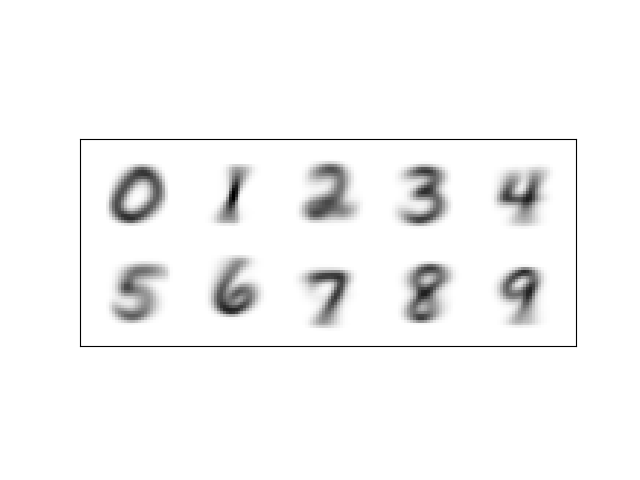
\includegraphics[width=0.5\textwidth]{../code_and_data/mle.png}
        \caption{The MLE estimator $\theta$ for each class.}
    \end{figure}

    \item Since we are to use a uniform prior for $\pi$, we have that 
    
    \begin{align*}
        \argmax_\pi \log(p(\pi | \mathcal{D})) &= \argmax_\pi \log\left(\frac{p(\pi) p(\mathcal{D} | \pi)}{p(\mathcal{D}}\right)\\
        &= \argmax_\pi \log\left(p(\pi)\right) + \log \left(p(\mathcal{D} | \pi)\right) - \log(p(\mathcal{D}))\\
    \end{align*}

    Since $p(\mathcal{D})$ is a constant with respect to $\pi$, and $p(\pi)$ is also a constant with respect to $\pi$ (uniform prior), we have that 

    \[\pi_{MAP} = \argmax_\pi \log(p(\pi | \mathcal{D})) = \argmax_\pi \log(p(\mathcal{D} | \pi)) = \pi_{MLE}\]

    and so the MAP estimator for $\pi$ is the same as the MLE estimator for $\pi$, which is given by 

    \[\pi_j =  \frac{N_{c = k}}{N}\]

    where $N_{c = k}$ is the number of examples with class $c = k$.

    However, the MAP estimator for $\theta$ is different from the MLE estimator for $\theta$. It is computed by 

    \begin{align*}
        \argmax_{\theta} \log(p(\theta | \mathcal{D})) &= \argmax_{\theta} \log\left(\frac{p(\theta) p(\mathcal{D} | \theta)}{p(\mathcal{D})}\right)\\
        &= \argmax_{\theta} \log\left(p(\theta)\right) + \log \left(p(\mathcal{D} | \theta)\right)
    \end{align*}

    Now, we know that 

    \begin{align*}
        \log\left(p(\theta)\right) + \log \left(p(\mathcal{D} | \theta)\right) &= \log\left(
        \prod_{c, j} \theta_{j, c}^{\alpha - 1} (1 - \theta_{j, c})^{\beta - 1} \right)
        + \log \left(p(\mathcal{D} | \theta)\right) \\
        &= \sum_{c, j} \left[(\alpha - 1) \log(\theta_{j, c}) + (\beta - 1) \log(1 - \theta_{j, c})\right] + \log \left(p(\mathcal{D} | \theta)\right) \\
    \end{align*}

Taking the partial derivative with respect to $\theta_{j, c}$, we get

    \begin{align*}
        \frac{\partial}{\partial \theta_{j, c}} &= \frac{\alpha - 1}{\theta_{j, c}} - \frac{\beta - 1}{1 - \theta_{j, c}} + \frac{\partial}{\partial \theta_{j, c}} \log \left(p(\mathcal{D} | \theta)\right) \\
        &= \frac{\alpha - 1}{\theta_{j, c}} - \frac{\beta - 1}{1 - \theta_{j, c}} + \frac{N_{1, c}}{\theta_{j, c}} - \frac{N_{0, c}}{1 - \theta_{j, c}} \\
        &= \frac{N_{1, c} + \alpha - 1}{\theta_{j, c}} - \frac{N_{0, c} + \beta - 1}{1 - \theta_{j, c}} \\
        &= 0
    \end{align*}

    and now solving for $\theta_{j, c}$, we get

    \[\theta_{j, c} = \frac{N_{1, c} + \alpha - 1}{N_{0, c} + N_{1, c} + \alpha + \beta - 2}\]

    \item Done in the code. Here are the statistics:
    
    \begin{verbatim}
        Average log-likelihood for MAP is  -173.46659721464317  (not normalized)
        Training accuracy for MAP is  0.8352166666666667
        Test accuracy for MAP is  0.816
    \end{verbatim}

    I am not normalizing the log-likelihood for each example $i$ in class $c$ by subtracting $\log(p(x | \theta, \pi))$, since this is a constant with respect to $c$ and so does not change the predictions. Further, this is hard to compute, as it is given by 
    
    \[\log(p(x | \theta, \pi)) = \log\left(\sum_{c = 1}^k p(x | \theta, \pi, c) p(c | \theta, \pi)\right)\]

    which is a logarithm of a sum, which cannot be computed by the logarithms of the summands. In general, it was mentioned in lecture and tutorial that computing this is intractable. I have submitted, however, the code that computes it -- it is only commented out.

    \item Here's the picture:
    
    \begin{figure}[H]
        \centering
        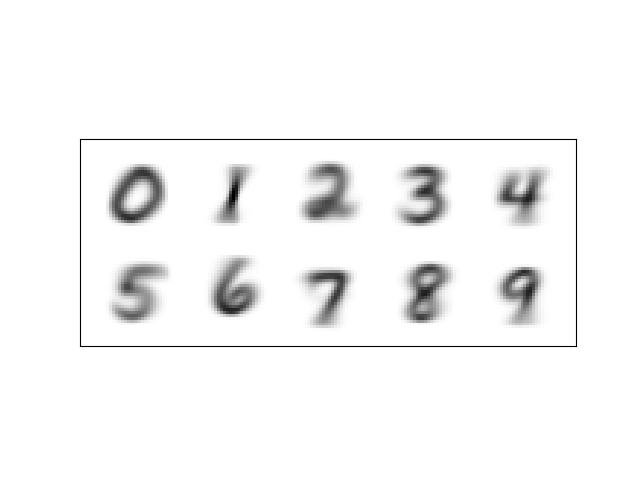
\includegraphics[width=0.5\textwidth]{../code_and_data/map.png}
        \caption{The MAP estimator $\theta$ for each class.}
    \end{figure}

    \item An advantage of the Naive Bayes approach is that since parameters are assumed to be independent of each other, we can optimize them independently of each other. In this case, we were able to compute a closed-form solution for $\theta$ and $\pi$ for both MLE and MAP, producing very fast training times. 
    
    A disadvantage of the Naive Bayes approach is that it assumes that the features are independent of each other, which is not the case in this problem. For example, in the case of the MNIST dataset, the pixels are not independent of each other, as it is likely that a pixel is white given that neighbouring pixels are also white. This is not captured by the Naive Bayes approach. 

\end{enumerate}

\newpage 
\section*{Question 3: Logistic Regression with Gaussian Prior}

\begin{enumerate}[(a)]
    \item First, let's write down an expression for the log likelihood of $\theta$. 
    
    \begin{align*}
        ll(\theta) &= \log(p(\mathcal{D} | \theta)) \\
        &= \log\left(\prod_{i = 1}^N \sigma((x^{(i)})^T \theta)^{y^{(i)}} (1 - \sigma((x^{(i)})^T \theta))^{1 - y^{(i)}}\right)\\
        &= \sum_{i = 1}^N y^{(i)} \log(\sigma((x^{(i)})^T \theta)) + (1 - y^{(i)}) \log(1 - \sigma((x^{(i)})^T \theta))
    \end{align*}

    This is optimized by gradient descent by taking the gradient with respect to $\theta$ to perform gradient descent. We get 

    \begin{align*}
        \nabla_\theta ll(\theta) &= \sum_{i = 1}^N y^{(i)} (1 - \sigma((x^{(i)})^T \theta)) x^{(i)} - (1 - y^{(i)}) \sigma((x^{(i)})^T \theta) x^{(i)} \\
        &= \sum_{i = 1}^N (y^{(i)} - \sigma((x^{(i)})^T \theta)) x^{(i)}
    \end{align*}

    and so we optimize (maximize) by performing gradient ASCENT with the update rule

    \[\theta_{t + 1} = \theta_t + \eta \sum_{i = 1}^N (y^{(i)} - \sigma((x^{(i)})^T \theta)) x^{(i)}\]

    \item The MAP log-likelihood of $\theta$ is given by 
    
    \begin{align*}
        ll_{MAP}(\theta) &= \log(p(\theta | D)) \\
        &= C_1 + \log(p(\theta) p(D | \theta))\\
        &= C_1 + \log\left(
            \frac{1}{(2\pi)^{d/2} |\Sigma|^{1/2}} \exp\left(-\frac{1}{2} \theta^T \Sigma^{-1} \theta \right)
        \right) + \log(p(D | \theta)) \\
        &= C_1 + C_2 + ll_{MLE}(\theta) + \log\left(\exp\left(-\frac{1}{2} \theta^T {(\sigma^2 I)}^{-1} \theta \right)
        \right) \\
        &= C_1 + C_2 + ll_{MLE}(\theta) -\frac{1}{2\sigma^2} \theta^T \theta \\
        &= C_1 + C_2 + ll_{MLE}(\theta) -\frac{1}{2\sigma^2} ||\theta||^2 \\
        &= C_1 + C_2 +  \sum_{i = 1}^N y^{(i)} \log(\sigma((x^{(i)})^T \theta)) + (1 - y^{(i)}) \log(1 - \sigma((x^{(i)})^T \theta)) - \frac{1}{2\sigma^2} ||\theta||^2
    \end{align*}

    where $C_1 = \log(p(D))$ and $C_2 = \log\left( \frac{1}{(2\pi)^{d/2} |\Sigma|^{1/2}} \right)$. 
\end{enumerate}

\end{document}